\begin{frame}{Определения косой информации Вигнера-Янасе в МК ЯМР (PLA-21)\footnote{S.I. Doronin, E.B. Fel'dman,  I.D. Lazarev, \textit{Phys. Lett. A} \textbf{406}, 127458 (2021)}}
  \begin{block}{Термодинамическое равновесное начальное состояние системы}
    \centering
    $
      \rho(0) = \rho_\mathrm{eq} = \frac{\exp(\frac{\hbar \omega_0}{kT}I_z)}{Z},
      \quad
      Z=Tr \left\{exp\left(\frac{\hbar \omega_0}{kT}I_z\right) \right\}
    $
  \end{block}

  Косая информация Вигнера-Янасе определяется как
  $$
  I_{WY}(\rho(\tau,\beta),I_z)
  = -2Tr([\sqrt{\rho(\tau,\beta)},I_z])^2.
  $$

  Эволюционная матрица плотности может быть представлена в виде
  $$
    \rho(\tau,\beta) = V^+(\tau) \frac{e^{\beta I_z}}{Z}V(\tau), \quad V(\tau) = e^{iH_{MQ}\tau}.
  $$

  Используем взаимосвязь:
  $$
    \sqrt{\rho(\tau,\beta)} =
        \sqrt{V^+(\tau)\frac{e^{\beta I_z}}{Z}V(\tau)} =
            V^+(\tau) \frac{e^{\frac{\beta}{2}I_z}}{\sqrt{Z}}V(\tau).
  $$

\end{frame}
\note{
  We start with initial thermodynamic equilibrium density matrix.
  $\hbar$ and $k$ are the Plank and Boltzmann constants, respectively,
  $\omega_0$ is the Larmor frequency,
  $T$ is the temperature,
  and $I_z$ is the operator of the projection of the total spin angular momentum on the $z$-axis,
  which is directed along the strong external magnetic field.

  The Wigner–Yanase skew information is defined as presented.

  Now we use the evident relationship:

  And now we can see that this part a similar to the evolution density matrix at double temperature.
}

\begin{frame}{Определения косой информации Вигнера-Янасе в МК ЯМР (PLA-21)}
Получаем
%
$$
    \left[I_z,\sqrt{\rho(\tau,\beta)}\right]
    = \left[I_z, \sum_k \rho_k \left(\tau, \frac{\beta}{2}\right)\right]
    = \sum_k k\rho_k \left(\tau, \frac{\beta}{2}\right)
$$
%
и
%
$$
	Tr\left[I_z,\sqrt{\rho(\tau,\beta)} \right]^2
	= Tr\left\{\sum_{k,k'}kk'
		\rho_k\left(\tau,\frac{\beta}{2}\right)
		\rho_{k'}\left(\tau,\frac{\beta}{2}\right)
	\right\}
	= \sum_k k^2 J_k\left(\tau,\frac{\beta}{2}\right).
$$


\begin{alertblock}{}
\centering
$
  I_{WY}\left(\rho(\tau, \beta), I_z\right)
  = 2\sum_k k^2 J_k\left(\tau, \frac{\beta}{2}\right)
  = 2M_2\left(\tau, \frac{\beta}{2}\right)
$
\end{alertblock}

\end{frame}
\note{
  Then we have ... and ...
  Thus, we obtain an important observation.
  If the spin system is investigated with MQ NMR at the temperature $T \approx \beta^{−1}$
  then the Wigner–Yanase skew information equals to the double second moment
  of the distribution of the intensities of the MQ NMR coherences at the temperature $2T \approx 2\beta^{−1}$
  at any time during the spin evolution.
  The Wigner–Yanase skew information is connected with the second moment of the distribution
  of the MQ NMR coherences analogously to the Fisher information.
  Lets compare these informations.
}

\begin{frame}{Определения косой информации Вигнера-Янасе в МК ЯМР (PLA-21)}
  \begin{columns}
  \column{0.4\textwidth}
  %\vspace{-3mm}
  \begin{figure}
    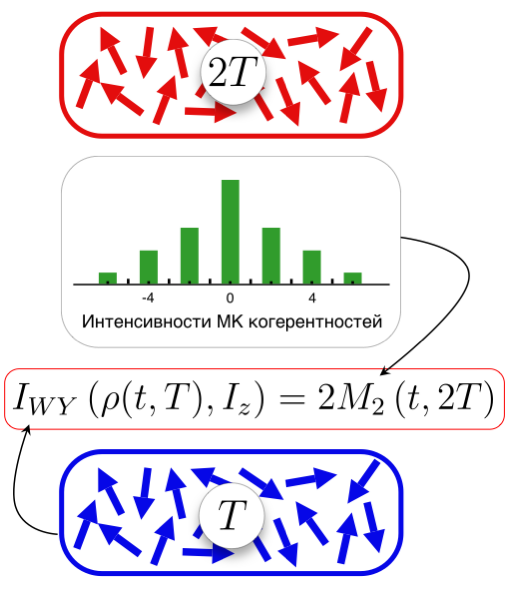
\includegraphics[width=0.9\textwidth]{wy-infromation-determination-cycle.png}
  \end{figure}
  \column{0.5\textwidth}
  Косая информация Вигнера-Янасе в системе с дипольным взаимодействием в МК эксперименте ЯМР при температуре T
  определяется\footnote[frame]{S. I. Doronin, E. B. Fel'dman,  I. D. Lazarev, \textit{Phys. Lett. A}, \textbf{406}, 127458 (2021)}
  удвоенным вторым моментом распределения МК когерентностей ЯМР при температуре 2T.
  \end{columns}
\end{frame}


\begin{frame}{Результаты: многочастичная запутанность (PLA-21)}
  \begin{columns}
    \column{0.5\textwidth}
    \begin{figure}
    \centering
    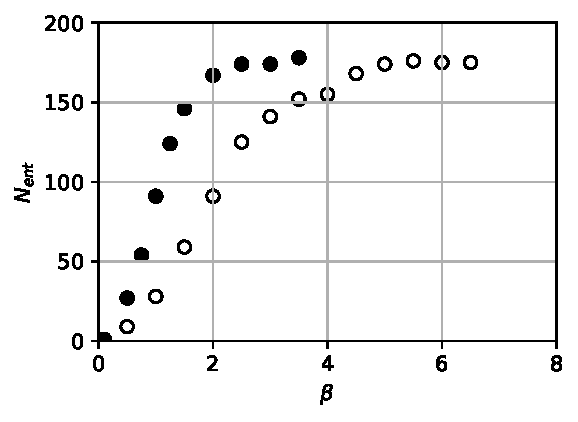
\includegraphics[width=0.9\textwidth]{result-nanopore-eq-nent-by-beta-qfi-wyi}
    \caption{Зависимость числа запутанных частиц от обратной температуры $\beta=\frac{\hbar\omega_0}{kT}$.}
    \end{figure}


    \column{0.4\textwidth}
    \begin{block}{}
      \vspace{-2mm}
      $$
      I_{WY}\left(\rho(\tau, \beta), I_z\right)
      = 2M_2\left(\tau, \frac{\beta}{2}\right)
      $$

      $$
        F_Q\left(\rho(\tau, \beta)\right)
        \geq 2M_2\left(\tau, \beta \right)
      $$
      \vspace{0.1mm}
    \end{block}
    \begin{block}{}
      Связь косой информации Вигнера-Янасе и информации
      Фишера\footnote[frame]{S.Luo, Proc.Amer. Math.Soc. 132, No.885-890 (2003)}:
      $$
      I_{WY}\left(\rho, I_z\right)
      \leq I_F\left(\rho, I_z\right)
      \leq 2I_{WY}\left(\rho, I_z\right)
      $$
      \vspace{0.1mm}
    \end{block}
  \end{columns}
\end{frame}
\note{
  The restrictions allow us to hope that the obtained results for the number of the entangled spins are not very
  different.
  For the comparison we used the model~\cite{23} of a nonspherical nanopore filled with a gas of spin-carrying atoms
  (for example, xenon) or molecules in a strong external magnetic field.
  This model allows the investigation of the many-spin entanglement in the spin system consisting of hundreds of nuclear
  spins~\cite{8}.

  We investigated many-spin entanglement in the spin system, consisting of 201 spins, in a nanopore both with
  the Wigner--Yanase information $I_{WY}\left(\rho(\tau, \beta), I_z\right)$
  and the Fisher information $I_F\left(\rho(\tau,\beta),I_z\right)$.
  In Fig. the dependence of the number of the entangled spins on the inverse temperature is presented.
  black circles - the results are obtained with the Fisher information
  open circles - the results are obtained with the Wigner–Yanase information.
  Fig.~\ref{fig:2} demonstrates that the number of the entangled spins increases when the temperature decreases both for
  the Wigner--Yanase information and the Fisher information.
}
